\documentclass[11pt,a4paper,twoside]{report}
\usepackage[utf8]{inputenc}
\usepackage{amsmath}
\usepackage{amsfonts}
\usepackage{amssymb}
\usepackage{graphicx}
\usepackage{fancyhdr}
\usepackage{listings}
\renewcommand{\bibname} {REFERENCES}
\usepackage[T1]{fontenc}
\usepackage{lmodern}
\usepackage{geometry}
\usepackage{textcomp}



\title{
\vspace{-3.4cm}
\begin{center}
%{\Large First Progress Report}\\
{\Large {\textbf{SOFTWARE DESIGN DOCUMENT}}  }\\
{\Large {\textbf{ON}}}\\
\textsf{\textbf{\Large{{GUIDANCE PERFORMANCE ANALYSIS FOR   }}}}\\
\vspace{0.01 cm}
\textsf{\textbf{\Large{{BLIND NAVIGATION SYSTEM USING  }}}}\\
\vspace{0.01 cm}
\textsf{\textbf{\Large{{NEURAL LEARNING IMAGE RECOGNITION}}}}\\
\vspace{0.2cm}
\begin{small}
 Submitted By :
 \end{small}
\begin{center}
\begin{large}
{AJITHKUMAR AK\hspace{13mm}EPAMEIT003}\\
{AKHIL A{\hspace{32mm}}EPAMEIT004}\\
{ARAVIND RAVINDRAN\hspace{3mm}EPAMEIT016}\\
{JITHIN S\hspace{32mm}EPAMEIT033}\\
{KIRAN TS\hspace{29mm}EPAMEIT034}\\
\end{large}
\end{center}
{\Large Guided By : }
{\textbf{\large Mr. RANJITH K }}\\
\begin{small}
(Asst.Prof. Department of Information Technology)
\end{small}
\end{center}
\vspace{0.05cm}
\begin{figure}[htbp]
\begin{center}

\includegraphics[scale=0.2]{emblem1.jpg}
\end{center}
\end{figure}
\begin{center}
%\vspace{0.25 cm}
{\Large Department of Information Technology} \\
%\vspace{0.015 cm}
{\Large Government Engineering College, Sreekrishnapuram}\\
%\vspace{0.015 cm}
{\large PALAKKAD - 678633}\\
%\vspace{0.25cm}
%{\large February, 2014}
%\tableofcontents
\end{center}
}
\begin{document}
\maketitle
\newpage
\pagenumbering{roman}
\setcounter{page}{0}

 
%===========================================================
\pagenumbering{roman}
\setcounter{page}{0}
\tableofcontents
%========================================================
\listoffigures
%========================================================
\chapter{INTRODUCTION}
\pagenumbering{arabic}

\pagestyle{fancy}
\rhead{\thepage}
\chead{}
\lhead{\textit{GUIDANCE PERFORMANCE ANALYSIS FOR BLIND NAVIGATION SYSTEM USING NEURAL LEARNING IMAGE RECOGNITION}}

\lfoot{\textit{Dept.Of Information Technology, Govt.Engg.College,Sreekrishnapuram }}
\cfoot{}
\rfoot{}
\renewcommand{\headrulewidth}{0.4pt}
\renewcommand{\footrulewidth}{0.4pt}

\paragraph{ }According to survey done India is now home to the world’s largest number of blind people. Of the 37 million people across the globe who are blind, over 15 million are from India. So in India blindness is the biggest problem. The leading causes of blindness are cataract, uncorrected refractive errors, glaucoma, and macular degeneration. Our goal is to create a portable, self-contained system that will allow visually impaired individuals to travel through familiar and unfamiliar environments without the assistance of guides and to recognize persons in front of the blind with the help of a smartphone. We uses a technology called Neural Network for image recognition. A key priority of this system is to meet the users navigation needs while ensuring low cost and portability embedded it with a Smartphone. The camera of the smartphone  is used to take real time images in front of the user, detect faces, process these faces using Neural Network and analyze it and finally recognize the face in front of him. A database consisting of images  is compared with the images captured at real time and suitable results is obtained.
%=====================================================================================================
%========================================================================================================
\chapter{SOFTWARE SPECIFICATIONS}
\section{SYSTEM REQUIREMENTS}
\begin{itemize}
\item Microsoft® Windows® 8.1/10 (32 or 64-bit).
\item 2 GB RAM minimum.
\item 400 MB hard disk space.
\item At least 1 GB for Android SDK, emulator system images, and caches.
\item 1280 x 800 minimum screen resolution.
\item Java Development Kit (JDK) 7.
\item Optional for accelerated emulator: Intel® processor with support for Intel® VT-x, Intel® EM64T (Intel® 64), and Execute Disable (XD) Bit functionality.

\end{itemize}
\section{SOFTWARE SECTION}
\begin{itemize}
\item Android SDK version 18 or higher: It is the software development kit developed
by android which helps developers to create software.
\item Google API: It is the application programming interface provided by google in
which developers can interface their application with google services like google
map etc.
\item TTS: It is another application service provided by the android which helps to
convert text into speech.
\item Android studio 5.0: It is the SDK which helps android programming easier.
\item OpenCV.
\end{itemize}
\section{HARDWARE SECTION}
\begin{itemize}
\item Arduino UNO : It is micro-controller which is used in the hardware part which
receives information from ultrasonic sensor and sends this data to a Smartphone
via a Bluetooth module attached to it.
\item Ultrasonic sensor (HC-SR04): It is an ultrasonic sensor which detects obstacles
in-front of the user and gives information to the micro-controller attached to it.
\item Bluetooth module (HC-06): It is connected to the micro-controller, sends instructions
to the Smartphone whenever obstacle is detected in-front of the user.
\item Smartphone: Any Smartphone which has android OS can be used which has access
to the Google services and have a compass inbuilt in it.


\end{itemize}
%=======================================================================================================
\chapter{INSTALLATION STEPS}
\section{INSTALL JDK AND ANDROID STUDIO}
\begin{itemize}
\item Download and Install JDK, SDK and Android Studio 5.0
\end{itemize}
\section{Set up OpenCV in android studio}

\begin{enumerate}
\item Download latest OpenCV sdk for Android from OpenCV.org and decompress the zip file.
\item Import OpenCV to Android Studio, From File -> New -> Import Module, choose sdk/java folder in the unzipped opencv archive.
\item Update build.gradle under imported OpenCV module to update 4 fields to match your project build.gradle
\begin{enumerate}
	\item[a] compileSdkVersion
	\item[b] buildToolsVersion
	\item[c] minSdkVersion
	\item[d] targetSdkVersion
\end{enumerate} 
\item Add module dependency by Application -> Module Settings, and select the Dependencies tab. Click + icon at bottom, choose Module Dependency and select the imported OpenCV module.
\begin{itemize}
\item[*] For Android Studio v1.2.2, to access to Module Settings : in the project view, right-click the dependent module $->$ Open Module Settings.
\end{itemize}
\item Copy libs folder under sdk/native to Android Studio under app/src/main.
\item 	In Android Studio, rename the copied libs directory to jniLibs and we are done. Step (6) is since Android studio expects native libs in app/src/main/jniLibs instead of older libsfolder.

\end{enumerate}


\section{INSTALL ARDUINO}
\begin{itemize}
\item Download and Install the Arduino Software.
\item Plug the Arduino into the PC.
\item Start the Windows Device Manager.
\item Install the	 Device Driver.
\item Setting up the Arduino Software.
\item Testing the Installation.

\end{itemize}

%=======================================================================================================
\chapter{MATHEMATICAL MODEL}

\section{PERCEPTRON}
\paragraph{ }In machine learning, the perceptron is an algorithm for supervised learning of binary classifiers: functions that can decide whether an input (represented by a vector of numbers) belongs to one class or another.[2] It is a type of linear classifier, i.e. a classification algorithm that makes its predictions based on a linear predictor function combining a set of weights with the feature vector. The algorithm allows for online learning, in that it processes elements in the training set one at a time.\\
\begin{center}
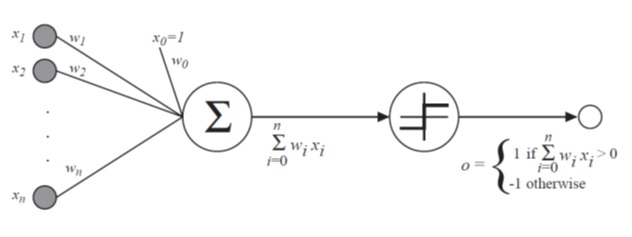
\includegraphics[scale=.75]{per.jpg}
\end{center}
It takes the inputs:
\begin{itemize}
\item $\sum_{i=0}^{n}w_ix_i =w_0x_0+w_1x_1+....+w_nx_n  $
\item $w_0$ denotes a threshold value
\item $x_0$ always 1
\end{itemize}
It outputs 1, if the result is greater than 1, otherwise -1
\paragraph{ }It can be used also for non-separable data sets, where the aim is to find a perceptron with a small number of misclassifications. However, these solutions appear purely stochastically and hence the pocket algorithm neither approaches them gradually in the course of learning, nor are they guaranteed to show up within a given number of learning steps.
\paragraph{ }Perceptron trainning rule
\begin{itemize}
\item uses thresholded unit
\item converges after a finite number of iterations
\item output hypothesis classifies training data perfectly
\item linearly separability necessary
\end{itemize}
\section{MULTILAYER PERCEPTRON }
\paragraph{ }It can be used also for non-separable data sets, where the aim is to find a perceptron with a small number of misclassifications. However, these solutions appear purely stochastically and hence the pocket algorithm neither approaches them gradually in the course of learning, nor are they guaranteed to show up within a given number of learning steps.
\begin{center}
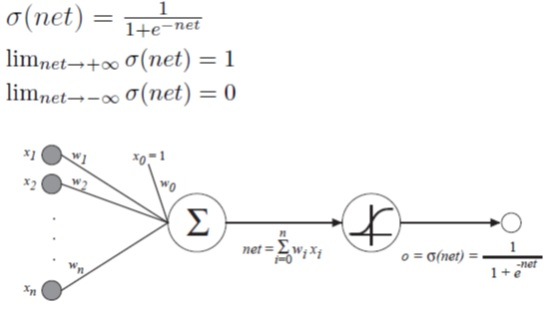
\includegraphics[scale=.75]{mlp.jpg}
\end{center}

\section{BACK PROPAGATION}
\paragraph{ }Learning occurs in the perceptron by changing connection weights after each piece of data is processed, based on the amount of error in the output compared to the expected result. This is an example of supervised learning, and is carried out through back propagation, a generalization of the least mean squares algorithm in the linear perceptron.
%=======================================================================================================
\chapter{PROPOSED ALGORITHM}
\begin{enumerate}

\end{enumerate}
%=======================================================================================================
\chapter{EXPECTED INPUT}
\begin{itemize}
\item Training inputs
\begin{enumerate}
\item Faces
\item Non faces
\item Desired faces
\end{enumerate}

\end{itemize}
\begin{figure}[htpb]
\begin{center}
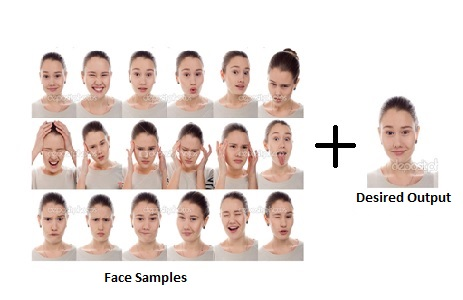
\includegraphics[scale=1]{input.jpg}
\caption{Expected inputs}
\end{center}
\end{figure}
\newpage
\begin{itemize}
\item Real time inputs
\begin{center}
\begin{figure}[htpb]
\center 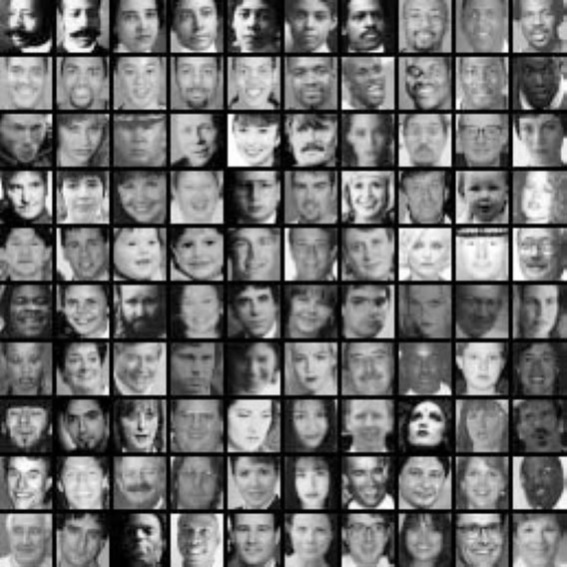
\includegraphics[scale=.5]{real}
\caption{Real time Inputs}
\end{figure}


\end{center}
\end{itemize}

%=======================================================================================================
\chapter{EXPECTED OUTPUT}
\begin{itemize}
\item Train Outputs
\begin{enumerate}
\item	The facial features converted to normalized values and these values stored in database
\item Fully trained neural network which is ready for real time testing.

\end{enumerate}
\end{itemize}
\begin{figure}[htpb]

\begin{center}
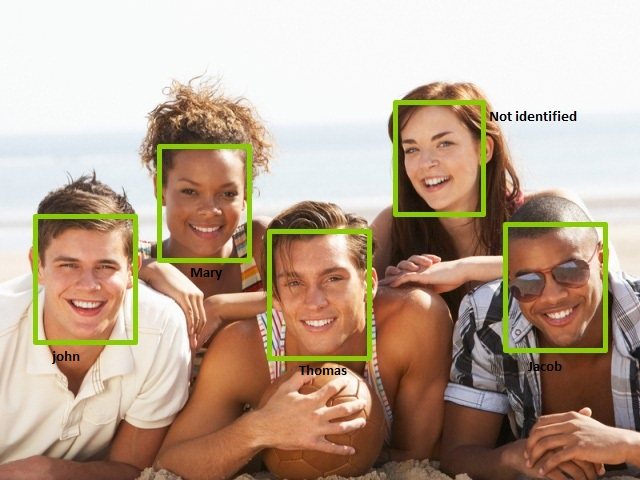
\includegraphics[scale=.5]{out}
\caption{Expected Output }
\end{center}

\end{figure}


\begin{itemize}
\item Real Time Output
\begin{enumerate}
\item If the person already in database then identify the person
\item If person not in database ask if want to add to database

\end{enumerate}

\end{itemize}


%=======================================================================================================
%=======================================================================================================
\addcontentsline{toc}{chapter}{REFERENCES}
\vspace{2pt}
\begin{thebibliography}{10}

\bibitem{key1}Zulhadi Zakaria, Nor Ashidi Mat Isa, and Shahrel A. Suandi. A study on neural network training algorithm for multiface detection in static images. volume 4 of 62, pages 170–173, Penang, Malaysia, February 2010. International Conference on Computer, Electrical, and Systems Science, and Engineering (ICCESSE 2010), World Academy of Science,
Engineering and Technology(WASET).


\vspace{1pt}
 \bibitem{key2}Guang Yi Ong, Zulhadi Zakaria, and Shahrel A. Suandi. Comparative
study on the influence of mahalanobis distance and skin color range for
face detection using adaboost. pages 5–8, Kuala Lumpur, May 2010. 2nd
International Conference on Electronic Computer Technology.


\vspace{1pt}
\bibitem{key3}Alexander Kuranov, Rainer Lienhart, and Vadim Pisarevsky. An empirical
analysis of boosting algorithms for rapid objects with an extended set of
haar-like features. Technical report, Intel Technical Report, July 02-01
2002.


\vspace{1pt}
\bibitem{key4}Gary Bradski, Adrian Kaehler, and Vadim Pisarevsky. Learningbased computer vision with Intel’s open source computer vision library. 9(2):119–130, May 2005.

\vspace{1pt}
\bibitem{key5}Minh-Tri Pham and Tat-Jen Cham. Fast training and selection of haar features using statistics in boosting-based face detection. In Minh-Tri Pham and Tat-Jen Cham, editors, none, volume 11 of none, page none, none, none 2007. IEEE International Conference on Computer Vision, none. none.

\vspace{1pt}
\bibitem{key6}Jack M Loomis, Reginald G, Roberta L . Navigation System for the Blind: Auditory Modes and Guidance . Presence Vol. 7,No 2, April 1998,193-203 c 1998 by the Massachusetts Institute of Technology.
\end{thebibliography}

%=======================================================================================================

\end{document}